	
\chapter*{Differential Equations with Boundary Conditions}
\addcontentsline{toc}{chapter}{Differential Equations with Boundary Conditions}  
\section*{More Python}
\addcontentsline{toc}{section}{More Python}  

\begin{problem} \label{P2.1}Work through Chapter 2 of Introduction to Python, where you will learn about lists, loops, and logic.
\end{problem}
\section*{Initial conditions vs. boundary conditions}
\addcontentsline{toc}{section}{Initial conditions vs. boundary conditions}  
In Physics 330, we studied the behavior of systems where the initial conditions were specified and we calculated how the system evolved forward in time (e.g. the f light of a baseball given its initial position and velocity). In these cases we were able to use Matlab\rq s convenient built-in differential equation solvers to model the system. The situation becomes somewhat more complicated if instead of having initial conditions, a differential equation has boundary conditions specified at both ends of the interval (rather than just at the beginning). This seemingly simple change in the boundary conditions makes it hard to use canned ODE solvers like Matlab\rq s ode45. Fortunately, there are better ways to solve these systems.

\section*{Solving differential equations with linear algebra}
\addcontentsline{toc}{section}{Solving differential equations with linear algebra} 

Consider the differential equation

\begin{equation} \label{eq:21}
	y^{\prime\prime}(x) + 9y(x) = sin(x) ; y(0) = 0, y(2) = 1
\end{equation}

\marginpar{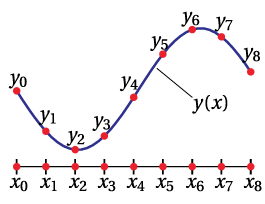
\includegraphics[width=\marginparwidth]{fig8}\captionof{figure}{A function $y(x)$ represented onacell-edge x-grid with $N=9$.}\label{fig:8}}

Notice that this differential equation has boundary conditions at both ends of the interval instead of having initial conditions at $x = 0$. If we represent this equation on a grid, we can turn this differential equation into a set of algebraic equations that we can solve using linear algebra techniques. Before we see how this works, let\rq s first specify the notation that we\rq ll use. We assume that we have set up a cell-edge spatial grid with N grid points, and we refer to the x values at the grid points using the notation $x_n$, with $n = 0..N−1$. We represent the(as yet unknown) function values $y(xn)$ on our grid using the notation $yn = y(xn)$. Now we can write the differential equation in finite difference form as it would appear on the grid. The second derivative in Eq. \ref{eq:21} is rewritten using the centered difference formula (see Eq. \ref{eq:5}), so that the finite difference version of Eq. \ref{eq:21} becomes:

\begin{equation} \label{eq:22}
	\frac{y_{n+1}-2y_n+y_{n-1}}{h^2}+9y_n = sin(x_n)
\end{equation}


Now let\rq s think about Eq.\ref{eq:22} for a bit.First notice that it is not an equation, but a system of many equations.We have one of these equations at every grid point n, except the end points j=0 and at j=N−1 where this formula reaches beyond the ends of the grid and cannot,therefore,be used.Because this equation involves $y_{n−1}$,$y_n$,and $y_{n+1}$ for the interior grid points n=1...N−2, Eq.(2.2) is really a  system of N−2 coupled equations in the N unknowns $y_0$ ...$y_{N−1}$.If we had just two more equations we could find the $y_n$\rq s by solving a linear system of equations. But we do have two more equations; they are the boundary conditions:
\begin{equation} \label{eq:23}
	y_0 = 0 ; y_{N-1} = 1
\end{equation}

which completes our system of N equations in N unknowns.\\
 Before Python can solve this system we have to put it in a matrix equation of the form

\begin{equation} \label{eq:24}
	A_y=b,
\end{equation}
where A is a matrix of coefficients, y the column vector of unknown y-values, and b the column vector of known values on the right-hand side of Eq.\ref{eq:22}.For the particular case of the system represented by Eqs.\ref{eq:22} and \ref{eq:23} ,the matrix equation is given by


\begin{equation} \label{eq:25}
	\begin{bmatrix}
		1 & 0 & 0 & 0 & ... & 0 & 0 & 0 \\
		\frac{1}{h^2} & -\frac{2}{h^2}+9 & \frac{1}{h^2} & 0 & ... & 0 & 0 & 0 \\
		0 &\frac{1}{h^2} & -\frac{2}{h^2}+9 & \frac{1}{h^2} & ... & 0 & 0 & 0 \\
		. & . & . & . & ... & .& . &. \\
		. & . & . & . & ... & .& . &. \\
		. & . & . & . & ... & .& . &. \\
		0 & 0 & 0 & 0 & ... & \frac{1}{h^2} & -\frac{2}{h^2}+9 & \frac{1}{h^2} \\
		0 & 0 & 0 & 0 & ... & 0 & 0 & 1  \\
	\end{bmatrix}
	\begin{bmatrix}
	y_0 \\ 
	y_1 \\ 
	y_2 \\ 
	. \\
	. \\
	. \\
	y_{N-2} \\ 
	y_{N-1} \\ 
	\end{bmatrix}
	=
	\begin{bmatrix}
		0 \\ 
		sin(x_1) \\
		sin(x_2) \\
		. \\
		. \\
		. \\
		sin(x_{N-2}) \\
		1 \\
	\end{bmatrix}
\end{equation}

Convince yourself that Eq.\ref{eq:25} is equivalent to Eqs. \ref{eq:22} and  \ref{eq:23} by mentally doing each row of the matrix multiply by tipping one row of the matrix up on end,dotting it into the column of unknowny-values, and setting it equal to the corresponding element in the column vector on the right. Once we have the finite-difference approximation to the differential equation in this matrix form $(Ay=b)$, a simple linear solve is all that is required to find the solution array $y_n$. NumPy can do this solve with the command linalg.solve(a,b).

\begin{problem} \label{P2.2}
\begin{enumerate}[label=(\alph*)]
	\item  Setup a cell-edge grid with $N=30$ grid points, like this: 
	\begin{lstlisting}	
	import numpy as np 
	N=30     #thenumberofgridpoints 
	a=0 
	b=2 
	x,h=np.linspace(a,b,N,retstep=True)
	\end{lstlisting}	
	 Look over this code and make sure you understand what it does before just using it.
	\item If you solve Eq. \ref{eq:21} analytically, you find
	\begin{equation}
	y(x) = \frac{16sin(3x)+cos(6-x)-cos(6+x)+cos(2+3x)-cos(2-3x)}{16sin(6)}
\end{equation}		
		Type this solution formula into the Python program that defines the grid above andplot the exact solution as a blue curve on a cell-edge grid with N points.
\marginpar{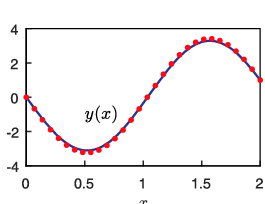
\includegraphics[width=\marginparwidth]{fig9}\captionof{figure}{The solution to 2.2(c) with N = 30}\label{fig:9}}

		\item Now create a matrix A filled with zeros using np.zeros, and write a for loop to load A like the matrix in Eq. \ref{eq:25} and do the linear solve to obtain $y_n$ and plot it on top of the exact solution with red dots ('r.') to see how closely the two agree. Experiment with larger values of N and plot the difference between the exact and approximate solutions to see how the error changes with N. We think you\rq ll be impressed at how well the numerical method works, if you use enough grid points.
\end{enumerate}
\end{problem}

Let\rq s pause a moment to review how to apply this technique to solve a problem. First, write out the differential equation as a set of finite difference equations on a grid, as we did in Eq. \ref{eq:22}. Then translate this set of finite difference equations (plus the boundary conditions) into a matrix form analogous to Eq. \ref{eq:25}. Finally, build the matrix A and the column vector y in Python and solve for the vectory. Our example, Eq. \ref{eq:21}, had only a second derivative, but first derivatives can be handled using the centered first derivative approximation, Eq. \ref{eq:5}. Let\rq s practice this procedure for a couple more differential equations:
\begin{problem} \label{P2.3}
	\begin{enumerate}[label=(\alph*)]
		\item Write out the finite difference equations on paper for the differential equation
		\marginpar{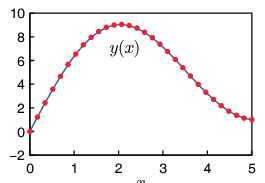
\includegraphics[width=\marginparwidth]{fig10}\captionof{figure}{Solution to 2.3(a) with N =30 (dots) compared to the exact solution (line)}\label{fig:10}}
		\begin{equation} \label{eq:26}
				y^{\prime\prime} + \frac{1}{x}y^\prime + (1 - \frac{1}{x^2})y=x ; y(0) = 0 , y(5) = 1
		\end{equation}
		Then write down the matrix A and the vector b for this equation. Finally, build these matrices in a Python program and solve the equation using the matrix method. Compare the solution found using the matrix method with the exact solution
		\begin{equation*}
			y(x) = \frac{-4}{J_1(5)}J_1(x)+x
		\end{equation*}
		$J_1(x)$ is the first order Bessel function.\\ HINT: When creating your b vector, you\rq ll be tempted to write some code like this: $b=x$. Don\rq t. This code just assigns b to be a reference to the matrix x. What you want is to create a copy of the matrix like this: \\ 
		\begin{lstlisting}	
	b = np.copy(x)
	\end{lstlisting}
	\item 	Solve the differential equation
	\begin{equation}\label{eq:27}
	y^{\prime\prime} + sin(x)y^\prime+e^xy=x^2 ; y(0) = 0, y(5)=3
\end{equation}		
	in Python using the matrix method. Mathematica\rq s NDSolve command claims that, to 15-digit accuracy
		\begin{equation*}
			y(4.5) = 8.720623277763513
		\end{equation*}

		\marginpar{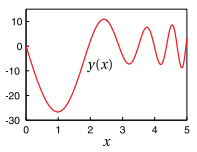
\includegraphics[width=\marginparwidth]{fig24}\captionof{figure}{Solution to 2.3(b) with N = 200} \label{fig:11}}
	You\rq d run out of memory with the matrix method long before achieving this level of accuracy, but how many points do you have to use in your numerical method to get agreement with Mathematica to 3 digits of accuracy (i.e. $y(4.5) = 8.72$)?		
		\\
		Hint: If your step size variable is h, the index for the for element where
$x_j \approx 4.5$ can be found this way:
	\begin{lstlisting}
		j = int(4.5/h)
	\end{lstlisting}
	The int command rounds the result and casts it as an integer so you can use it to access a specific element.
	\end{enumerate}
\end{problem}
	
\section*{Derivative boundary conditions}
\addcontentsline{toc}{section}{Derivative boundary conditions} 
\marginpar{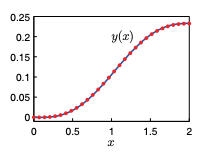
\includegraphics[width=\marginparwidth]{fig25}\captionof{figure}{The solution to $2.4$ (a) with $N=30$. The RMS difference from the exact solution is $8.8 \times 10^{-4}$}\label{fig:12}}

	Now let\rq s see how to modify the linear algebra approach to differential equations
so that we can handle boundary conditions where derivatives are specified instead
of values. Consider the differential equation
	\begin{equation}\label{eq:28}
		y^{\prime\prime}(x) + 9y(x) = x   ;    y(0) = 0,    Y^\prime(2) = 0
	\end{equation}
	We can satisfy the boundary condition $y(0) = 0$ as before (just use $y_1 = 0$), but
what do we do with the derivative condition at the other boundary?
\begin{problem} \label{P2.4}

\begin{enumerate}[label=(\alph*)]
\item	A crude way to implement the derivative boundary condition is to use a forward difference formula for the last two points:
	\begin{equation*}
		\frac{y_{N-1}-y_{N-2}}{h} = y^\prime\vert_{x=2}
	\end{equation*}
	
	In the present case, where $y^\prime(2) = 0$, this simply means that we need to write the last row of our matrix to enforce
	\begin{equation*}
		y_{N-1}-y_{N-2}= 0
	\end{equation*}
	Think about what the new boundary conditions will do to the final row of matrix A and the final element of vector b, and then solve Eq. \ref{eq:28} using the matrix method with this boundary condition. Compare the resulting numerical solution to the analytic solution:
	\begin{equation*}
		y(x) = \frac{x}{9} - \frac{\sin(3x)}{27\cos(6)}
	\end{equation*}
	\marginpar{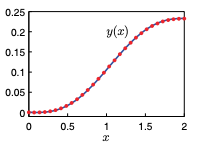
\includegraphics[width=\marginparwidth]{fig26}\captionof{figure}{The solution to $2.4$ (b) with $N=30$. The RMS difference from the exact solution is $5.4 \times 10^{-4}$}\label{fig:13}}

	\item You can improve the boundary condition formula using quadratic extrapolation. In this method, you fit a parabola of the form
	\begin{equation}\label{eq:29}
		y(x) = a+bx+cx^2
	\end{equation}
	
	to the last three points on your grid to find a, b, and c in terms of your data points. Then you take the derivative of Eq. \ref{eq:28} and evaluate it at
the edge $x = x_{N−1}$. Normally we\rq d make you go through the math to
derive this, but since time is short, we\rq ll just tell you that this process
gives you the following finite difference approximation for the $y^\prime(x)$ at
the end of the grid:
	\begin{equation}\label{eq:210}
		\frac{1}{2h} y_{N-3} - \frac{2}{h} y_{N-2} + \frac{3}{2h} y_{N-1} = y^\prime(X_{N-1})
	\end{equation}
Modify your program from part (a) to include this new condition and
show that it gives a more accurate solution than the crude technique of
part (a). When you check the accuracy, don\rq t just look at the end of the
interval. All of the points are coupled by the matrix A, so you should
use a full-interval accuracy check like the RMS (root-mean-square)
error:
\begin{lstlisting}
np.sqrt(np.mean((y-yexact)**2))
\end{lstlisting}
\end{enumerate}
\end{problem}

\section*{Nonlinear differential equations}
\addcontentsline{toc}{section}{Nonlinear differential equations} 
Finally, we must confess that we have been giving you easy problems to solve,
which probably leaves the impression that you can use this linear algebra trick
to solve all second-order differential equations with boundary conditions at the
ends. The problems we have given you so far are easy because they are linear
differential equations, so they can be translated into linear algebra problems.
Linear problems are not the whole story in physics, of course, but most of the
problems we will do in this course are linear, so these finite-difference and matrix
methods will serve us well in the labs to come.
	\marginpar{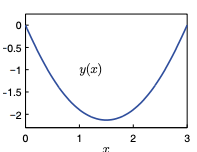
\includegraphics[width=\marginparwidth]{fig27}\captionof{figure}{The solution to $2.5(\mathrm{~b})$.}\label{fig:14}}
	\begin{problem} \label{P2.5}
\begin{enumerate}[label=(\alph*)]
\item Here is a simple example of a differential equation that isn\rq t linear:

	\begin{equation}\label{eq:211}
		y^{\prime\prime}(x) + \sin[y(x)] = 1 ; y(0) = 0, y(3) = 0
	\end{equation}
		Work at turning this problem into a linear algebra problem to see why
it can\rq t be done, and explain the reasons to the TA.
\item Let\rq s find a way to use a combination of linear algebra and iteration
(initial guess, refinement, etc.) to solve Eq. \ref{eq:211} in Python on a grid.
First, write the equation as
\begin{equation}\label{eq:212}
		y^{\prime\prime}(x)= 1 - \sin[y(x)]
	\end{equation}
	Make a guess for $y(x)$. It doesn\rq t have to be a very good guess. In this
case, the guess $y(x) = 0$ works just fine. Then treat the whole right side
of Eq.\ref{eq:212} as known so it goes in the b vector. Then you can solve the equation to find an improved guess for
$y(x)$. Use this better guess to rebuild b (again treating the right side of Eq. \ref{eq:212} as known), and
then re-solve to get and even better guess. Keep iterating until your $y(x)$ converges to the desired level of accuracy. This happens when your $y(x)$  satisfies \ref{eq:212}  to a specified criterion, not when the change
in $y(x)$ from one iteration to the next falls below a certain level. Iterate until your RMS error is less than $10^{-5}$, as described in the hint below.
HINT: An appropriate error vector would be
\begin{lstlisting}
err = A@y-(1-np.sin(y))
\end{lstlisting}
(remember that @ is the matrix multiplication operator). Compare
this to Eq. \ref{eq:212}
 and convince yourself that the entire vector err will
be zero when the equation is exactly solved. We\rq ll compute the RMS
error at interior points only, like this
\begin{lstlisting}
rmserr = np.sqrt(np.mean(err[1:-2]**2))
\end{lstlisting}
because the end points don\rq t satisfy the differential equation. Use rmserr as your check condition.
\end{enumerate}
\end{problem}
